\begin{DoxyVerb}Commands are sent to the ezLCD though the serial interface, Commands are text based and end with a carrage return <b>cr</b>.<br>
\end{DoxyVerb}
 So if you send {\bfseries cls} ending with a {\bfseries cr} the device will clear the screen and return a {\bfseries cr} when the command is complete,\par
 some widgets take a bit of time (in the millsecond range) to complete so after sending a command allways wait for a {\bfseries cr} to comeback before sending another command.\par
 \par
 Minimal example will open the ez\-L\-C\-D port clear the screen and print 'Hello From Python' in red \par
  
\begin{DoxyImageNoCaption}
  \mbox{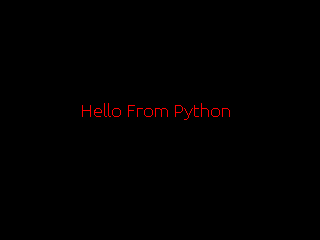
\includegraphics{minimal.png}}
\end{DoxyImageNoCaption}
 
\begin{DoxyCodeInclude}
1 \textcolor{comment}{# Minimal ezLCD Python demo}
2 \textcolor{comment}{#}
3 
4 \textcolor{keyword}{import} platform
5 \textcolor{keyword}{import} sys
6 
7 
8 sys.path.append(\textcolor{stringliteral}{"C:\(\backslash\)Users\(\backslash\)codeman\(\backslash\)Documents\(\backslash\)GitHub\(\backslash\)ezLCD3xxPython\(\backslash\)module"}) 
9 \textcolor{keyword}{from} ezLCD3xx \textcolor{keyword}{import} *
10 
11 \textcolor{comment}{#check what OS we are on}
12 \textcolor{comment}{#Windows}
13 \textcolor{keywordflow}{if} platform.system() == \textcolor{stringliteral}{'Windows'}:
14     LCD = ezLCD(\textcolor{stringliteral}{'com6'}) 
15 \textcolor{comment}{#Mac}
16 \textcolor{keywordflow}{elif} platform.system() == \textcolor{stringliteral}{'Dawrwin'}:
17     LCD = ezLCD(\textcolor{stringliteral}{'/dev/tty.usbsomething'})
18 \textcolor{comment}{# Bail out if comport error}
19 \textcolor{keywordflow}{if} LCD.openSerial()==\textcolor{keyword}{False}:
20     \textcolor{keywordflow}{print} \textcolor{stringliteral}{'Error Opening Port'}
21     \textcolor{keywordflow}{raise} SystemExit
22 
23 \textcolor{comment}{# Turn verbose off }
24 LCD.verbose(\textcolor{stringliteral}{'off'})
25 \textcolor{comment}{# Turn off button press info from ezLCD}
26 LCD.wquiet(ON)
27 \textcolor{comment}{# CLear screen}
28 LCD.cls()
29 \textcolor{comment}{# Set draw color to red}
30 LCD.color(RED)
31 \textcolor{comment}{# Print string at coordinates x=80 and y=100}
32 LCD.printString(\textcolor{stringliteral}{"Hello From Python"},80,100)
33 
\end{DoxyCodeInclude}
 Button example will display a button widget then poll for button presses and update screen \par
  
\begin{DoxyImageNoCaption}
  \mbox{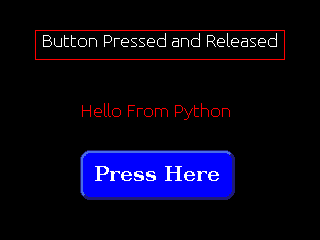
\includegraphics{button.png}}
\end{DoxyImageNoCaption}
 
\begin{DoxyCodeInclude}
1 \textcolor{comment}{# Button ezLCD Python demo}
2 \textcolor{comment}{#}
3 
4 \textcolor{keyword}{import} platform
5 \textcolor{keyword}{import} sys
6 
7 sys.path.append(\textcolor{stringliteral}{"C:\(\backslash\)Users\(\backslash\)segler\(\backslash\)Documents\(\backslash\)GitHub\(\backslash\)ezLCD3xxPython\(\backslash\)module"}) 
8 \textcolor{keyword}{from} ezLCD3xx \textcolor{keyword}{import} *
9 
10 \textcolor{comment}{#check what OS we are on}
11 \textcolor{comment}{#Windows}
12 \textcolor{keywordflow}{if} platform.system() == \textcolor{stringliteral}{'Windows'}:
13     LCD = ezLCD(\textcolor{stringliteral}{'com4'}) 
14 \textcolor{comment}{#Mac}
15 \textcolor{keywordflow}{elif} platform.system() == \textcolor{stringliteral}{'Dawrwin'}:
16     LCD = ezLCD(\textcolor{stringliteral}{'/dev/tty.usbsomething'})
17 \textcolor{comment}{# Bail out if comport error}
18 \textcolor{keywordflow}{if} LCD.openSerial()==\textcolor{keyword}{False}:
19     \textcolor{keywordflow}{print} \textcolor{stringliteral}{'Error Opening Port'}
20     \textcolor{keywordflow}{raise} SystemExit
21 
22 \textcolor{comment}{# Turn verbose off }
23 LCD.verbose(\textcolor{stringliteral}{'off'})
24 \textcolor{comment}{# Turn off button press info from ezLCD}
25 LCD.wquiet(ON)
26 \textcolor{comment}{# CLear screen}
27 LCD.cls()
28 \textcolor{comment}{# Set draw color to red}
29 LCD.color(RED)
30 \textcolor{comment}{# Set widget font 0}
31 LCD.fontw(0,\textcolor{stringliteral}{'1'})
32 \textcolor{comment}{# Set wodget font 1}
33 LCD.fontw(1,\textcolor{stringliteral}{'0'})
34 \textcolor{comment}{# Set theme #1 }
35 LCD.theme(1, 155, 152, 3, 0, 3, 24, 4, 5, 0, 1)
36 \textcolor{comment}{# Print string at coordinates x=80 and y=100}
37 LCD.printString(\textcolor{stringliteral}{"Hello From Python"},80,100)
38 \textcolor{comment}{# Draw button widget with a ID of 1}
39 LCD.button( 1,  80, 150, 155, 50, 1, 0, 10, 6, 3, \textcolor{stringliteral}{'Press Here'})
40 \textcolor{comment}{# Draw a staticText box}
41 LCD.staticText(2, 35, 30, 250, 30, 8, 1, 1,\textcolor{stringliteral}{'Press Button'})
42 \textcolor{comment}{# Clear widget stack}
43 LCD.wstack(CLEAR)
44 
45 \textcolor{keywordflow}{while} \textcolor{keyword}{True}:
46     \textcolor{comment}{# check widget stack this will return widget updates (button press ect.) last in first out order}
47     (ID, Info, Data) = LCD.wstack(LIFO)
48     \textcolor{comment}{# check if ID = 1 widget 1 and info = pressed }
49     \textcolor{keywordflow}{if} ID == 1 \textcolor{keywordflow}{and} Info == 4:
50         \textcolor{comment}{# clear the stack just to be safe}
51         LCD.wstack(CLEAR)
52         \textcolor{comment}{# change draw color to yellow}
53         LCD.color(YELLOW)
54         \textcolor{comment}{# change change string 1 for text on static text ID 2}
55         LCD.string(1,\textcolor{stringliteral}{'Button Pressed'})
56         \textcolor{comment}{# redraw static text box ID 2 3=redraw      }
57         LCD.wstate(2, 3)
58     \textcolor{comment}{# check if ID = 1 widget 1 and info = pressed and released}
59     \textcolor{keywordflow}{if} ID == 1 \textcolor{keywordflow}{and} Info == 1:
60         \textcolor{comment}{# clear the stack just to be safe}
61         LCD.wstack(CLEAR)
62         \textcolor{comment}{# change draw color to yellow}
63         LCD.color(YELLOW)
64         \textcolor{comment}{# change change string 1 for text on static text ID 2}
65         LCD.string(1,\textcolor{stringliteral}{'Button Pressed and Released'})
66         \textcolor{comment}{# redraw static text box ID 2 3=redraw}
67         LCD.wstate(2, 3)
68 
69         
\end{DoxyCodeInclude}
 \begin{DoxyVerb}Load example will display the cpu load as a graph  <br>
\end{DoxyVerb}
  
\begin{DoxyImageNoCaption}
  \mbox{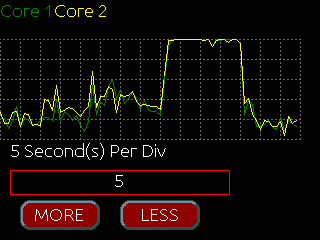
\includegraphics{load.png}}
\end{DoxyImageNoCaption}
 
\begin{DoxyCodeInclude}
1 \textcolor{comment}{#!/usr/bin/env python}
2 \textcolor{comment}{# Python Serial library for ezLCD3xx}
3 \textcolor{comment}{# http://www.ezlcd.com/}
4 \textcolor{comment}{#}
5 \textcolor{comment}{# You need the pySerial Library by Chris Liechti}
6 \textcolor{comment}{# http://pyserial.wiki.sourceforge.net/pySerial}
7 \textcolor{comment}{#}
8 
9 
10 \textcolor{comment}{# END SerLCD Class Definition --------------------------------------}
11 
12 \textcolor{comment}{# Start Test Program -----------------------------------------------}
13 \textcolor{keyword}{import} commands
14 \textcolor{keyword}{import} os
15 \textcolor{keyword}{import} re
16 \textcolor{keyword}{import} time \textcolor{keyword}{as} timer
17 \textcolor{keyword}{import} sys
18 \textcolor{keyword}{import} platform
19 \textcolor{keyword}{import} time
20 \textcolor{keyword}{import} psutil
21     
22 sys.path.append(\textcolor{stringliteral}{"C:\(\backslash\)Users\(\backslash\)codeman\(\backslash\)Documents\(\backslash\)GitHub\(\backslash\)ezLCD3xxPython\(\backslash\)module"}) 
23 \textcolor{keyword}{from} ezLCD3xx \textcolor{keyword}{import} *
24 
25 \textcolor{keyword}{def }drawGrid():
26     LCD.lineType(2)
27     LCD.xy(0,30)
28     LCD.color(BLACK)
29     LCD.box(300,110,1)
30     LCD.xy(0,0)
31     LCD.color(GREEN)
32     LCD.printString(\textcolor{stringliteral}{'Core 1'})
33     LCD.color(YELLOW)
34     LCD.printString(\textcolor{stringliteral}{'Core 2'})
35     LCD.color(155)
36     LCD.color(LIME)
37     LCD.font(\textcolor{stringliteral}{'1'})
38     LCD.font(\textcolor{stringliteral}{'0'})
39     LCD.color(151)
40     \textcolor{keywordflow}{for} y \textcolor{keywordflow}{in} range(6):
41         LCD.xy(0,(y*20)+39)
42         LCD.line(300,(y*20)+39)
43     \textcolor{keywordflow}{for} x \textcolor{keywordflow}{in} range(16):
44         LCD.xy(x*20,39)
45         LCD.line(x*20,139)
46     LCD.xy(300,39)
47     LCD.line(300,139)
48     LCD.lineType(0)
49     
50 \textcolor{keyword}{def }drawTime(res):
51     LCD.xy(10,140)
52     LCD.color(BLACK)
53     LCD.box(300,30, FILLED)
54     LCD.color(WHITE)
55     Time=str(res)+\textcolor{stringliteral}{' Second(s) Per Div'}
56     LCD.printString(Time)
57 
58     LCD.string(5, str(res))
59     LCD.wstate(7,REDRAW)
60 
61 
62 \textcolor{keywordflow}{if} platform.system() == \textcolor{stringliteral}{'Windows'}:
63     LCD = ezLCD(\textcolor{stringliteral}{'com6'}) 
64 \textcolor{keywordflow}{elif} platform.system() == \textcolor{stringliteral}{'Dawrwin'}:
65     LCD = ezLCD(\textcolor{stringliteral}{'/dev/tty.usbsomething'})
66 \textcolor{keywordflow}{if} LCD.openSerial()==\textcolor{keyword}{False}:
67     \textcolor{keywordflow}{print} \textcolor{stringliteral}{'Error Opening Port'}
68     \textcolor{keywordflow}{raise} SystemExit   
69     
70 LCD.verbose(\textcolor{stringliteral}{'OFF'})
71 LCD.wquiet(ON)
72 LCD.cls()
73 LCD.fontw(0,\textcolor{stringliteral}{'1'})
74 LCD.fontw(1,\textcolor{stringliteral}{'0'})
75 LCD.fontw(2,\textcolor{stringliteral}{'serif24'})
76 LCD.theme(1, 155, 152, 3, 0, 3, 24, 4, 5, 0, 1)
77 LCD.backlight(100, 5, 10)
78 LCD.cls()
79 LCD.font(\textcolor{stringliteral}{'0'})
80 LCD.fonto(0)
81 info = \textcolor{stringliteral}{' '}
82 LCD.string( 1, \textcolor{stringliteral}{'%'})
83 LCD.color(WHITE)
84 LCD.cfgio(8,\textcolor{stringliteral}{'analog'})
85 \textcolor{keywordflow}{print} LCD.xmax()
86 \textcolor{keywordflow}{print} LCD.ymax()
87 LCD.xy(100,100)
88 (x,y) = LCD.xy()
89 \textcolor{keywordflow}{print} int(x), int(y)
90 (r,g,b)=LCD.colorId(3)
91 \textcolor{keywordflow}{print} r,g,b
92 \textcolor{keywordflow}{print} LCD.string(65)
93 \textcolor{keywordflow}{print} LCD.string(66)
94 \textcolor{keywordflow}{print} LCD.color()
95 \textcolor{keywordflow}{print} LCD.io(8)
96 
97 
98 LCD.button( 5, 20, 200, 80, 30 , 1, 0, 10, 1, 2, \textcolor{stringliteral}{'MORE'})
99 LCD.button( 6, 120, 200, 80, 30 , 1, 0, 10, 1, 3, \textcolor{stringliteral}{'LESS'})
100 LCD.staticText(7, 10, 170, 220, 25, 8, 1, 5, \textcolor{stringliteral}{'test'})
101 drawGrid()
102 x=0
103 y1=239
104 y2=239
105 lx=0
106 ly1=239
107 ly2=239
108 res=5
109 drawTime(res)   
110 LCD.wstack(CLEAR)     
111 \textcolor{keywordflow}{while} \textcolor{keyword}{True}:
112 
113     oldinfo = info
114     cores=psutil.cpu\_percent(interval=1, percpu=\textcolor{keyword}{True})
115     y1 = 139 - cores[0]
116     y2 = 139 - cores[1]
117     \textcolor{keywordflow}{if} x!=0:
118         LCD.color(GREEN)
119         LCD.xy(lx,ly1)
120         LCD.line(x, y1)
121         LCD.color(YELLOW)
122         LCD.xy(lx,ly2)
123         LCD.line(x, y2)
124     ly1 = y1
125     ly2 = y2
126     lx = x   
127     x += 20/res
128     
129     \textcolor{keywordflow}{if} x >= 300:
130         x=0
131         y1=239
132         y2=239
133         lx =0
134         ly1 =239
135         ly2 =239
136         drawGrid()
137     (ID, info, data) = LCD.wstack(LIFO)
138     LCD.wstack(CLEAR)
139     \textcolor{keywordflow}{if} ID == 5 \textcolor{keywordflow}{and} info==1:
140         res +=1
141         drawTime(res)  
142     \textcolor{keywordflow}{if} ID == 6 \textcolor{keywordflow}{and} info==1:
143         \textcolor{keywordflow}{if} res > 1:
144             res -=1
145             drawTime(res)
146 LCD.closeSerial()
147 \textcolor{comment}{# End Test Program --------------------------------------}
\end{DoxyCodeInclude}
 